\documentclass[12pt]{article}

\usepackage[utf8]{inputenc} 
\usepackage[T1]{fontenc}   
\usepackage{hyperref}       
\usepackage{url}           
\usepackage{booktabs}       
\usepackage{amsfonts}       
\usepackage{amsmath}  
\usepackage{nicefrac}      
\usepackage{microtype}      
\usepackage{lipsum}
\usepackage{graphicx}
\usepackage{float}
\usepackage{indentfirst}
\usepackage{setspace}
\usepackage{geometry}
\usepackage{caption}
\usepackage{subcaption}
\usepackage{listings}
\usepackage{pgfplots}
\usepackage{adjustbox}
\geometry{
    a4paper,
    left=25mm,
    right=25mm,
    top=25mm,
    bottom=25mm
}

\begin{document}
\author{Jędrzej Szor 239716}
\title{\text{Obliczenia ewolucyjne}\\\textbf{Implementacja algorytmów MSPSO, MPSO oraz BOA}}
\maketitle

\section{Opis zaproponowanej wersji algorytmu BOA}
Zaimplementowana przeze mnie wersja algorytmu BOA bazuje na dokumencie zamieszczonym na wikampie. W na jedną iterację składa się obliczenie zapachu dla każdego motyla w roju, wybranie najlepszego osobnika oraz obliczenie nowych koordynatów dla każdego motyla. Zapach oblicza się na podstawie poniższych wzorów:
\begin{equation}
    f = cI^a
\end{equation}
\begin{equation}
    I = \frac{1}{F}
\end{equation}
gdzie $F$ jest wartością funkcji dla aktualnych współrzędnych motyla.\\
Zastosowany sposób obliczania zapachu podstawowego $I$ pozwala osiągnąć minimum globalne będące $\geq 0$. W przypadku globalnego minimum $\le 0$ pojawiają się liczby zespolone, w które się nie zagłębiałem.
\begin{figure}[H]
    \centering
    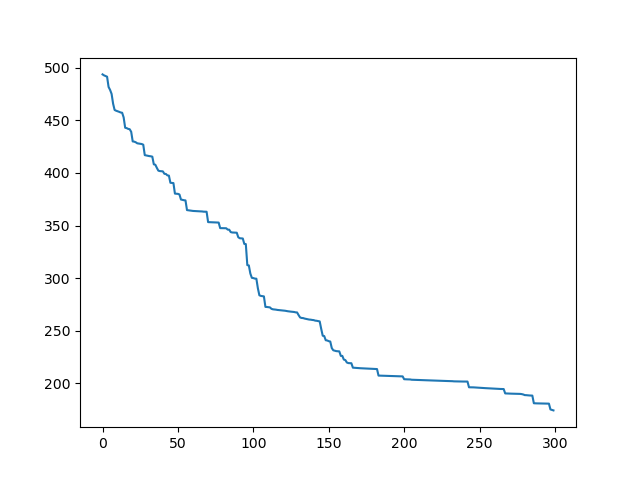
\includegraphics[width=10cm]{plots/BOA/1_best.png}
    \caption{Wykres najlepszych wartości dla funkcji sfery podniesionej o 10.}
\end{figure}
Poniżej zaprezentowane są wyniki przebiegu poszczególnych algorytmów z wybranymi wartościami parametrów. Wykresy zostały sporządzone na podstawie 30 przebiegów algorytmów po 500 iteracji dla dziedzin przewidzianych w dokumencie z opisami funkcji.
\begin{figure}[H]
    \centering
    \begin{subfigure}{0.32\textwidth}
        \centering
        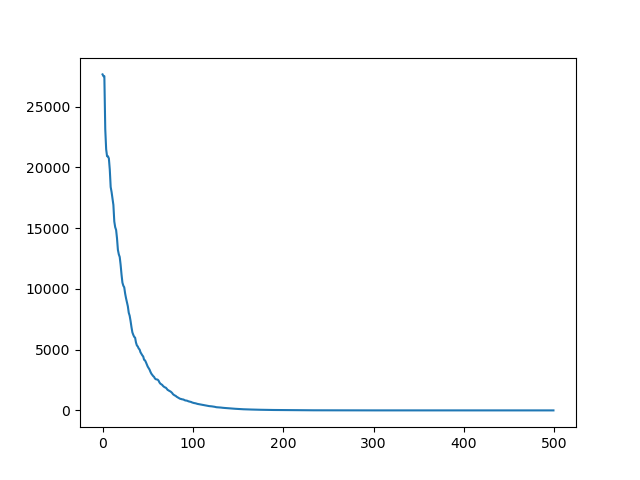
\includegraphics[width=\linewidth]{plots/MSPSO/sphere.png}
        \caption{MSPSO}
    \end{subfigure}
    \begin{subfigure}{0.32\textwidth}
        \centering
        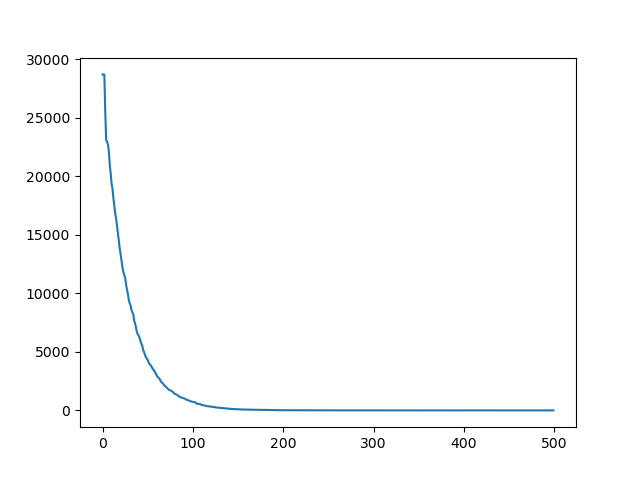
\includegraphics[width=\linewidth]{plots/MPSO/sphere.png}
        \caption{MPSO}
    \end{subfigure}
    \begin{subfigure}{0.32\textwidth}
        \centering
        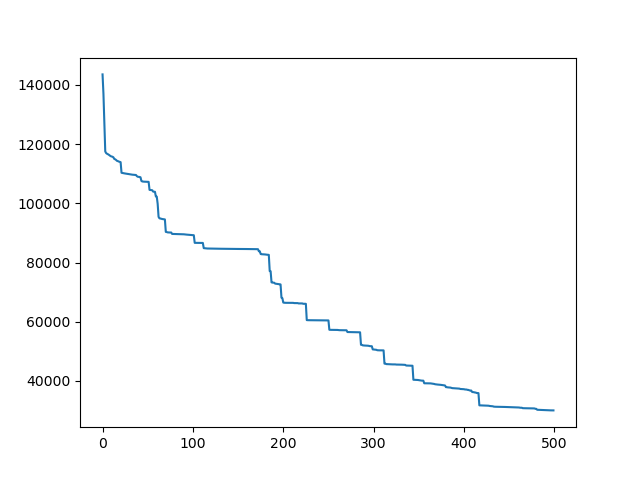
\includegraphics[width=\linewidth]{plots/BOA/sphere.png}
        \caption{BOA}
    \end{subfigure}
    \caption{Wyniki dla funkcji sfery}
\end{figure}
\begin{figure}[H]
    \centering
    \begin{subfigure}{0.32\textwidth}
        \centering
        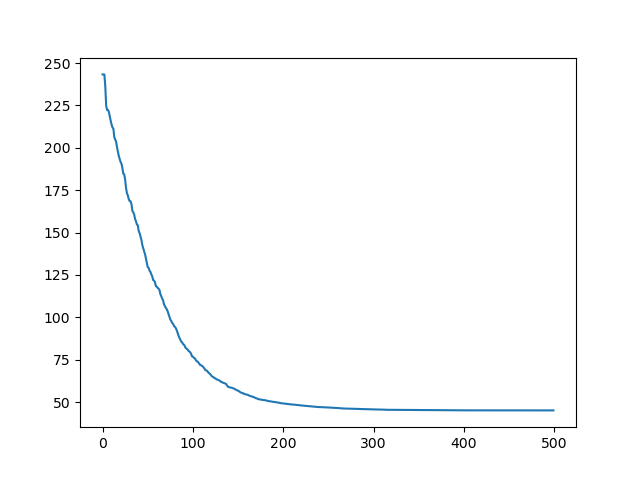
\includegraphics[width=\linewidth]{plots/MSPSO/rastrigin.png}
        \caption{MSPSO}
    \end{subfigure}
    \begin{subfigure}{0.32\textwidth}
        \centering
        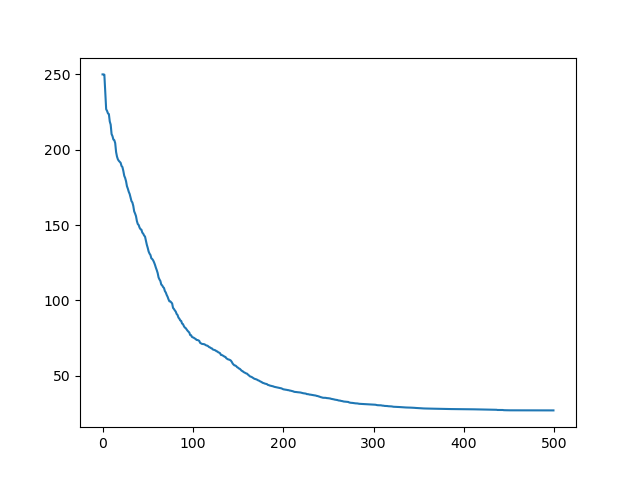
\includegraphics[width=\linewidth]{plots/MPSO/rastrigin.png}
        \caption{MPSO}
    \end{subfigure}
    \begin{subfigure}{0.32\textwidth}
        \centering
        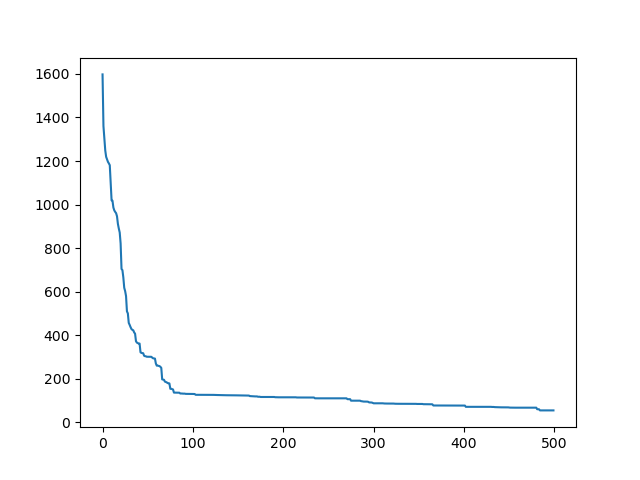
\includegraphics[width=\linewidth]{plots/BOA/rastrigin.png}
        \caption{BOA}
    \end{subfigure}
    \caption{Wyniki dla funkcji Rastrigina}
\end{figure}
\begin{figure}[H]
    \centering
    \begin{subfigure}{0.32\textwidth}
        \centering
        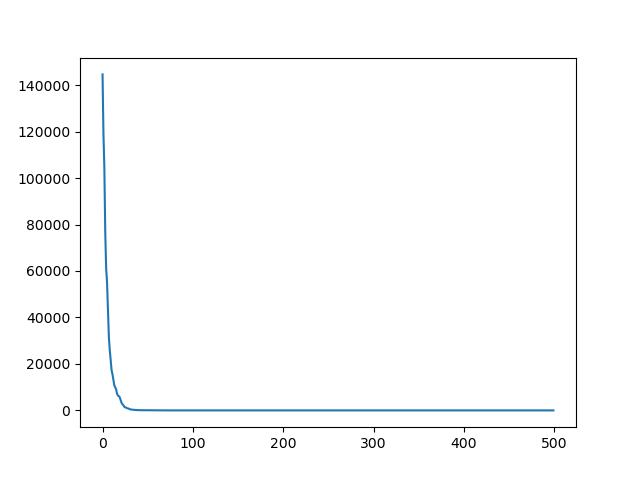
\includegraphics[width=\linewidth]{plots/MSPSO/corana.png}
        \caption{MSPSO}
    \end{subfigure}
    \begin{subfigure}{0.32\textwidth}
        \centering
        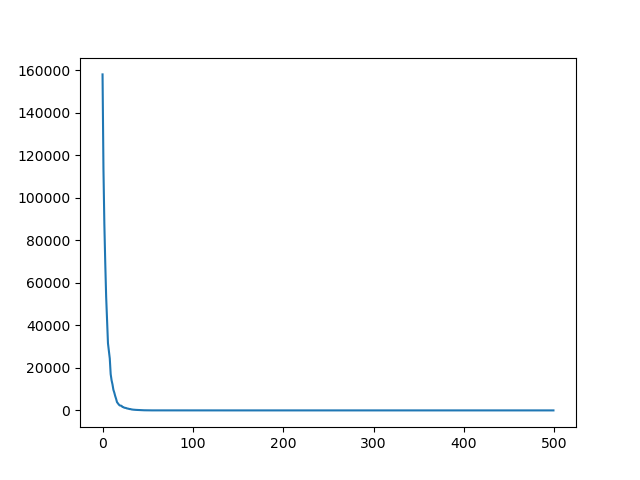
\includegraphics[width=\linewidth]{plots/MPSO/corana.png}
        \caption{MPSO}
    \end{subfigure}
    \begin{subfigure}{0.32\textwidth}
        \centering
        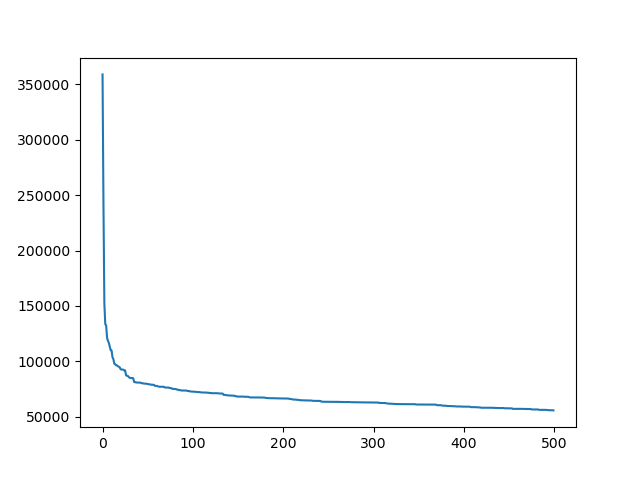
\includegraphics[width=\linewidth]{plots/BOA/corana.png}
        \caption{BOA}
    \end{subfigure}
    \caption{Wyniki dla funkcji Corany}
\end{figure}
Jak widać na wykresach, algorytmy MSPSO oraz MPSO są o wiele bardziej niezawodne. Algorytm BOA jest jednak wielokrotnie szybszy. Średni czas przebiegu dla BOA wynosił nieco powyżej minuty, podczas gdy czas wykonania pozostałych algorytmów wahał się pomiędzy 30 a 40 minut.

\section{Analiza wpływu parametrów na charakterystykę przebiegu algorytmów}
Wszystkie eksperymenty w niniejszej sekcji wykonane zostały na funkcji sfery dla 20 wymiarów, 300 iteracji oraz prezentują wyniki uśrednione z 30 przebiegów.

\subsection{MSPSO}
W algorytmach MSPSO oraz MPSO zastosowałem zmienne współczynniki przyspieszenia opisane szczegółowo w poprzednim raporcie.
\begin{gather}
    wt = wt_{min} + (wt_{max} - wt_{min})\frac{(t_{max} - t)}{t_{max}},\\
    c_1 = (c_{1f} - c_{1i})\frac{t}{t_{max}} + c_{1i},\\
    c_2 = (c_{2f} - c_{2i})\frac{t}{t_{max}} + c_{2i}
\end{gather}

\begin{itemize}
    \item $w_{init} = 0.9,\; w_{final} = 0.4$
    \item $c_{1init} = 2,\; c_{1final} = 1$
    \item $c_{2init} = 1,\; c_{2final} = 2$
\end{itemize}
\begin{figure}[H]
    \centering
    \begin{subfigure}{0.49\textwidth}
        \centering
        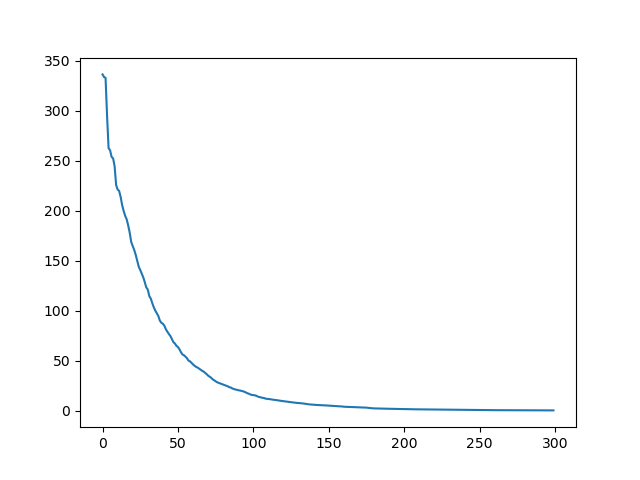
\includegraphics[width=\linewidth]{plots/MSPSO/1_best.png}
        \caption{Populacja = 10, min = $9.00\cdot 10^{-3}$, czas = 1m 43s}
    \end{subfigure}
    \begin{subfigure}{0.49\textwidth}
        \centering
        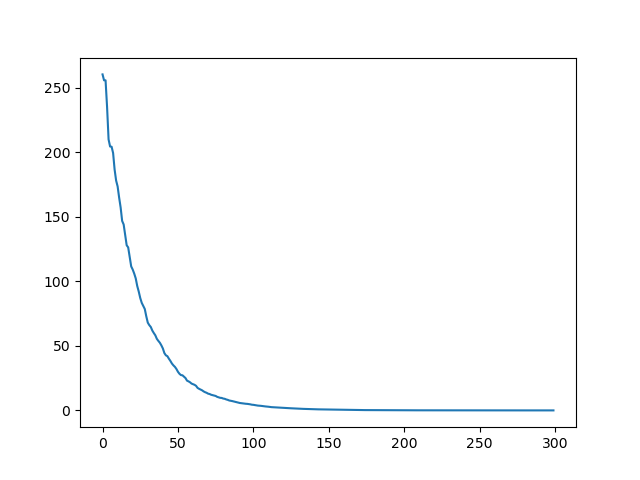
\includegraphics[width=\linewidth]{plots/MSPSO/2_best.png}
        \caption{Populacja = 30, min = $2.04\cdot 10^{-4}$, czas = 13m 36s}
    \end{subfigure}
    \caption{Wyniki dla zmiennej liczby populacji. Liczba rojów = 5}
\end{figure}

\begin{figure}[H]
    \centering
    \begin{subfigure}{0.49\textwidth}
        \centering
        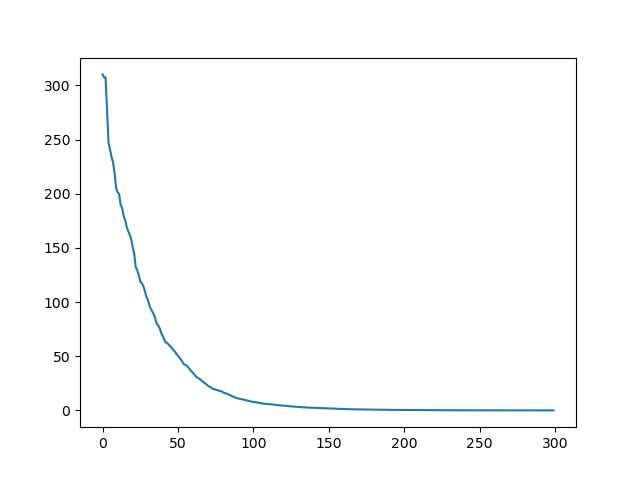
\includegraphics[width=\linewidth]{plots/MSPSO/3_best.png}
        \caption{Liczba rojów = 3, min = $1.30\cdot 10^{-3}$, czas = 3m 52s}
    \end{subfigure}
    \begin{subfigure}{0.49\textwidth}
        \centering
        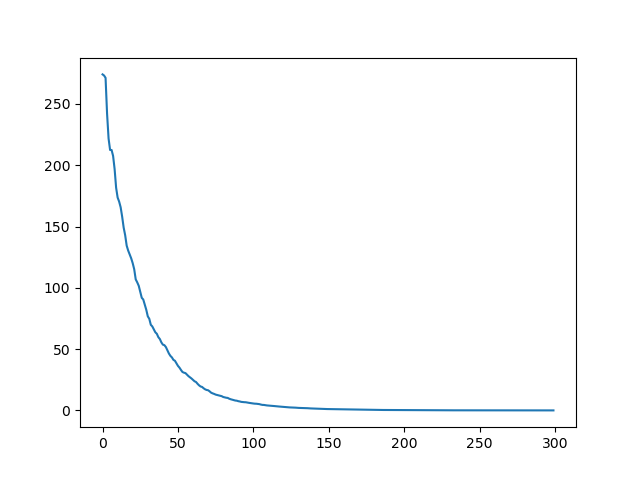
\includegraphics[width=\linewidth]{plots/MSPSO/4_best.png}
        \caption{Liczba rojów = 8, min = $2.04\cdot 10^{-3}$, czas = 10m 8s}
    \end{subfigure}
    \caption{Wyniki dla zmiennej liczby rojów. Populacja = 20}
\end{figure}
Jak widać na wykresach liczba populacji i rojów poprawia czas zbiegania do minimum, jednak ogromnym kosztem czasowym. Przy zmianach obu parametrów różnice w charakterystyce są znikome, podczas gdy czas wykonania jest kilkukrotnie dłuższy.

\subsection{MPSO}
\begin{figure}[H]
    \centering
    \begin{subfigure}{0.49\textwidth}
        \centering
        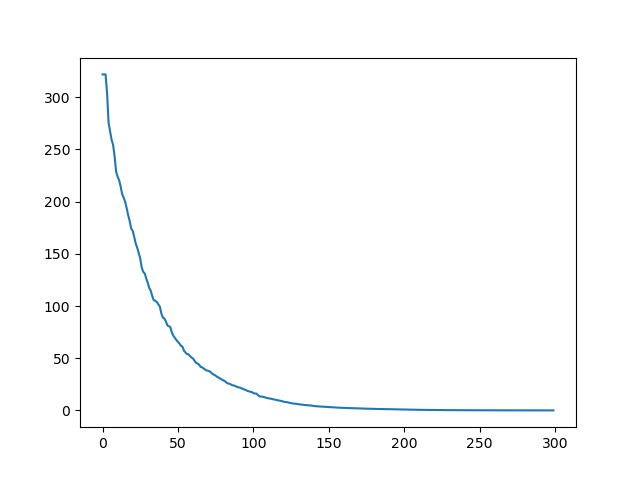
\includegraphics[width=\linewidth]{plots/MPSO/1_best.png}
        \caption{Populacja = 10, min = $7.08\cdot 10^{-3}$, czas = 1m 42s}
    \end{subfigure}
    \begin{subfigure}{0.49\textwidth}
        \centering
        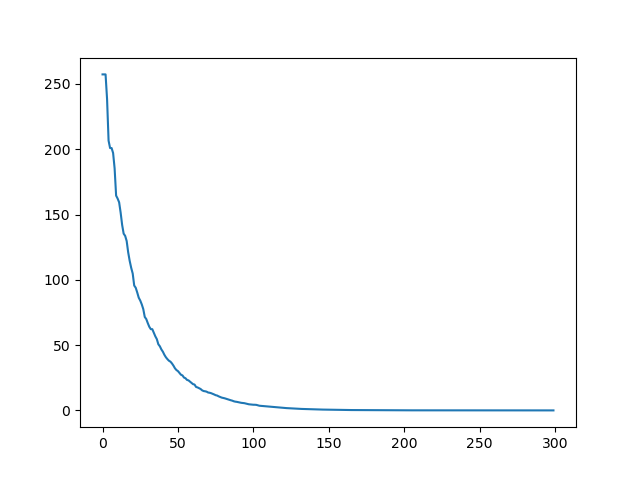
\includegraphics[width=\linewidth]{plots/MPSO/2_best.png}
        \caption{Populacja = 30, min = $3.72\cdot 10^{-4}$, czas = 13m 42s}
    \end{subfigure}
    \caption{Wyniki dla zmiennej liczby populacji. Liczba rojów = 5, tasowanie cząstek co 100 iteracji}
\end{figure}

\begin{figure}[H]
    \centering
    \begin{subfigure}{0.49\textwidth}
        \centering
        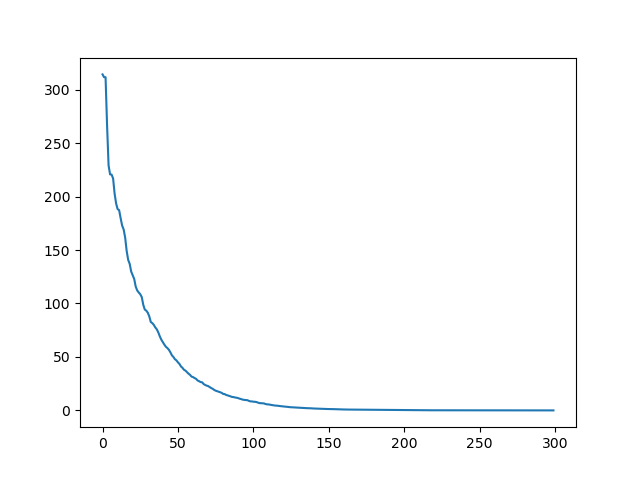
\includegraphics[width=\linewidth]{plots/MPSO/3_best.png}
        \caption{Liczba rojów = 3, min = $1.01\cdot 10^{-3}$, czas = 3m 50s}
    \end{subfigure}
    \begin{subfigure}{0.49\textwidth}
        \centering
        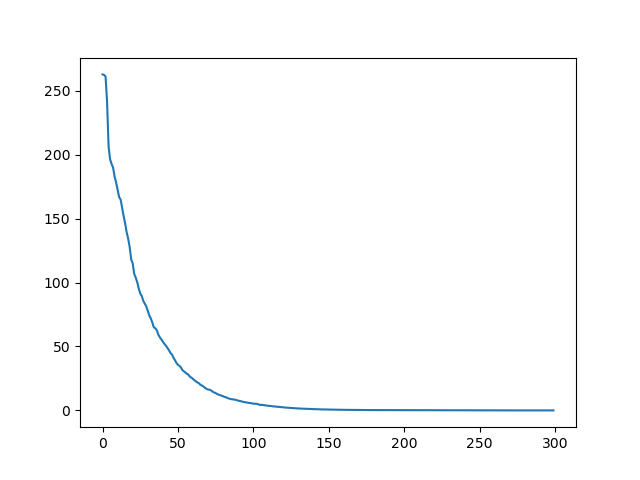
\includegraphics[width=\linewidth]{plots/MPSO/4_best.png}
        \caption{Liczba rojów = 8, min = $4.84\cdot 10^{-4}$, czas = 9m 57s}
    \end{subfigure}
    \caption{Wyniki dla zmiennej liczby rojów. Populacja = 20, tasowanie cząstek co 100 iteracji}
\end{figure}

\begin{figure}[H]
    \centering
    \begin{subfigure}{0.49\textwidth}
        \centering
        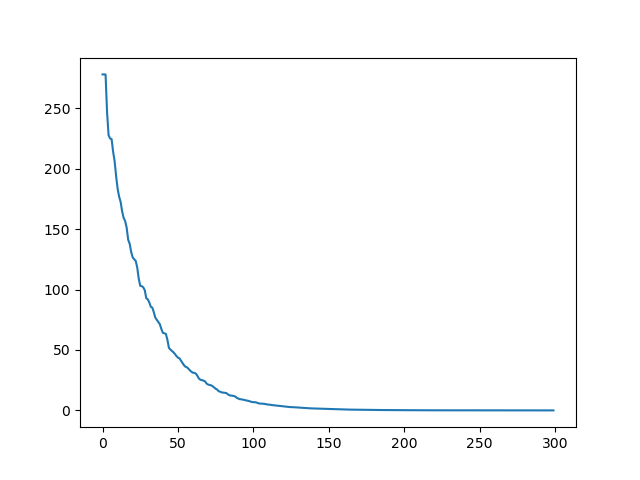
\includegraphics[width=\linewidth]{plots/MPSO/5_best.png}
        \caption{Tasowanie cząstek co 20 iteracji, min = $1.56\cdot 10^{-3}$, czas = 6m 17s}
    \end{subfigure}
    \begin{subfigure}{0.49\textwidth}
        \centering
        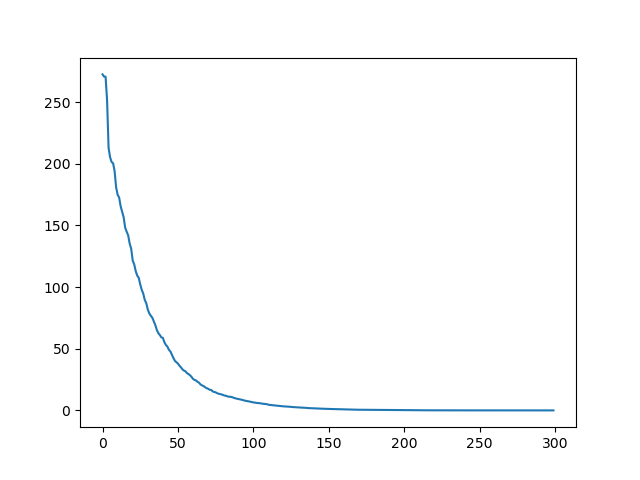
\includegraphics[width=\linewidth]{plots/MPSO/6_best.png}
        \caption{Tasowanie cząstek co 150 iteracji, min = $1.40\cdot 10^{-3}$, czas = 6m 9s}
    \end{subfigure}
    \caption{Wyniki dla zmiennej częstotliwości tasowania cząstek. Populacja = 20, liczba rojów = 5}
\end{figure}
Podobnie jak przy MSPSO, zmiany w charakterystykach podczas zmian ilości cząstek oraz ilości rojów są znikome, podczas gdy znacząco wydłuża się czas wykonania. Interesującym spostrzeżeniem jest to, że lepsze wyniki zostały uzyskane przy rzadszym tasowaniu cząstek.

\subsection{BOA}
Próbowałem różnych wersji zmiennego współczynnika $a$: Liniowo malejący od 1 do 0, liniowo malejący od 1 do 0.5, nieliniowo zmienny, jednak najlepsze efekty uzyskałem używając stałej wartości.
\begin{figure}[H]
    \centering
    \begin{subfigure}{0.49\textwidth}
        \centering
        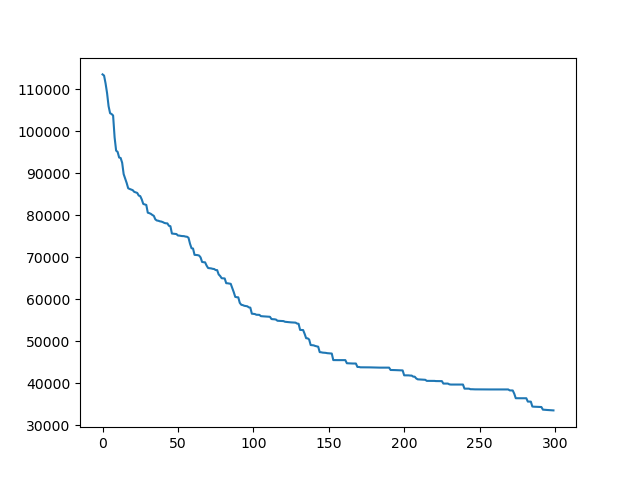
\includegraphics[width=\linewidth]{plots/BOA/2_best.png}
        \caption{Populacja = 20, min = $3.26\cdot 10^{-9}$, czas = 4s}
    \end{subfigure}
    \begin{subfigure}{0.49\textwidth}
        \centering
        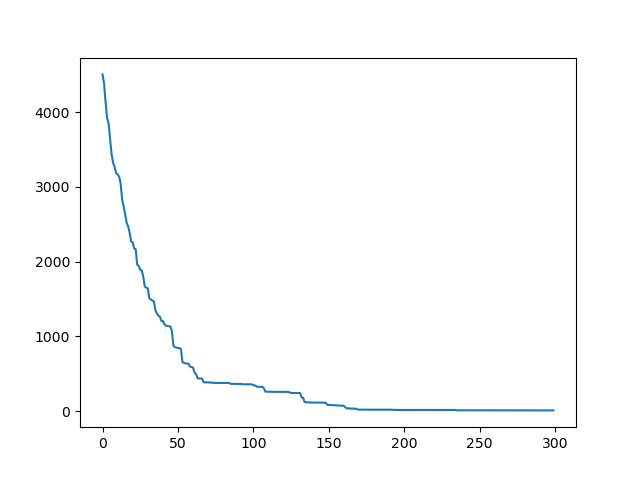
\includegraphics[width=\linewidth]{plots/BOA/3_best.png}
        \caption{Populacja = 50, min = $1.38\cdot 10^{-4}$, czas = 11s}
    \end{subfigure}
    \caption{Wyniki dla zmiennej liczby populacji. a = 0.5, c = 0.5, p = 0.5}
\end{figure}

\begin{figure}[H]
    \centering
    \begin{subfigure}{0.49\textwidth}
        \centering
        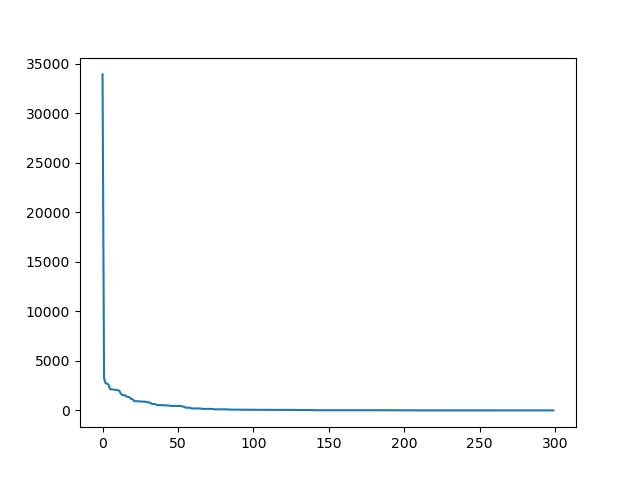
\includegraphics[width=\linewidth]{plots/BOA/4_best.png}
        \caption{p = 0.7, min = $6.37\cdot 10^{-5}$, czas = 7s}
    \end{subfigure}
    \begin{subfigure}{0.49\textwidth}
        \centering
        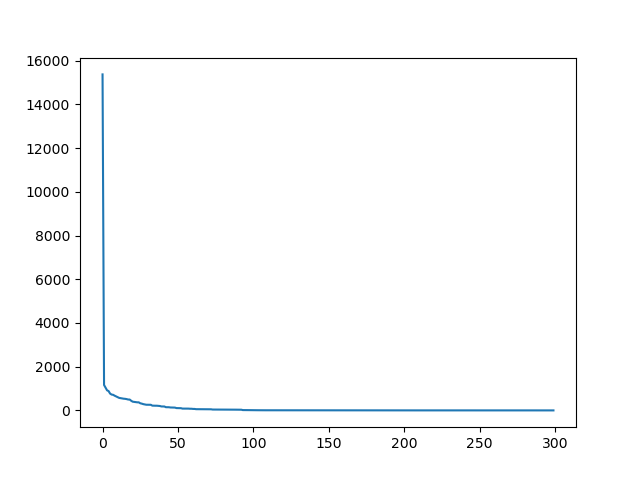
\includegraphics[width=\linewidth]{plots/BOA/5_best.png}
        \caption{p = 0.3, min = $3.26\cdot 10^{-5}$, czas = 8s}
    \end{subfigure}
    \caption{Wyniki dla zmiennego współczynnika p. a = 0.5, c = 0.5, populacja = 35}
\end{figure}

\begin{figure}[H]
    \centering
    \begin{subfigure}{0.49\textwidth}
        \centering
        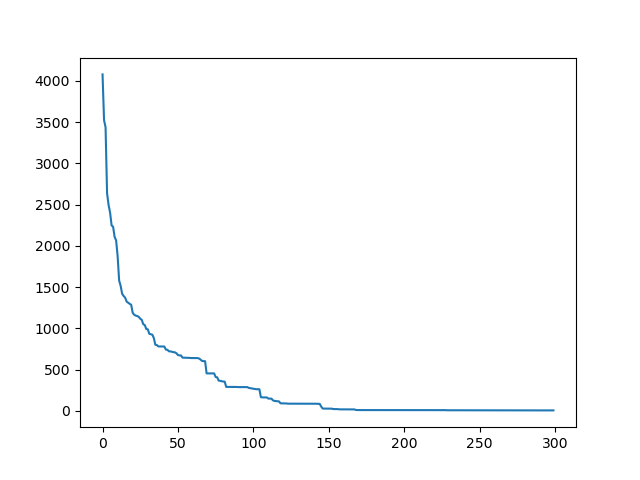
\includegraphics[width=\linewidth]{plots/BOA/6_best.png}
        \caption{c = 0.7, min = $5.01\cdot 10^{-5}$, czas = 7s}
    \end{subfigure}
    \begin{subfigure}{0.49\textwidth}
        \centering
        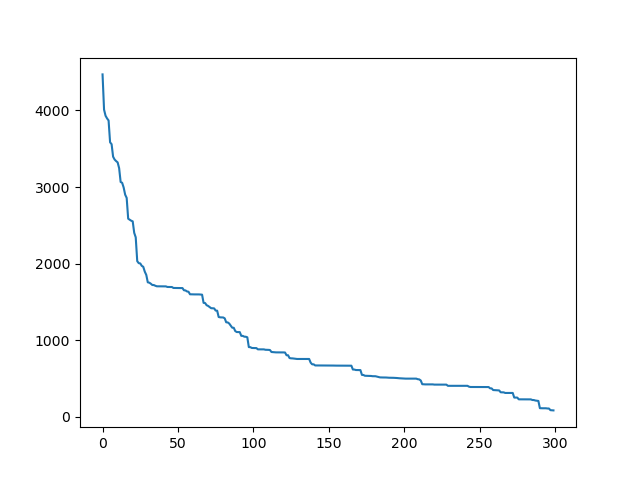
\includegraphics[width=\linewidth]{plots/BOA/7_best.png}
        \caption{c = 0.3, min = $4.73\cdot 10^{-6}$, czas = 6s}
    \end{subfigure}
    \caption{Wyniki dla zmiennego współczynnika c. a = 0.5, p = 0.5, populacja = 35}
\end{figure}

\begin{figure}[H]
    \centering
    \begin{subfigure}{0.49\textwidth}
        \centering
        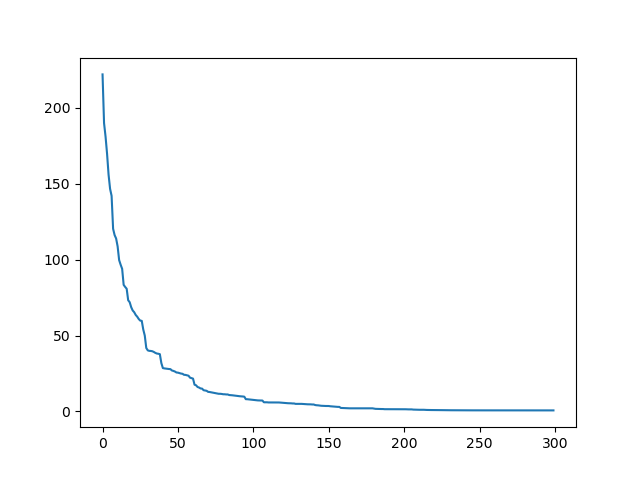
\includegraphics[width=\linewidth]{plots/BOA/8_best.png}
        \caption{a = 0.7, min = $8.76\cdot 10^{-4}$, czas = 7s}
    \end{subfigure}
    \begin{subfigure}{0.49\textwidth}
        \centering
        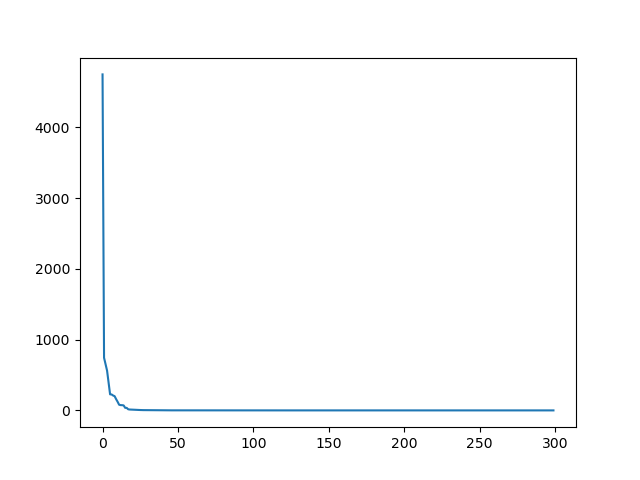
\includegraphics[width=\linewidth]{plots/BOA/9_best.png}
        \caption{a = 0.3, min = $8.03\cdot 10^{-9}$, czas = 7s}
    \end{subfigure}
    \caption{Wyniki dla zmiennego współczynnika a. c = 0.5, p = 0.5, populacja = 35}
\end{figure}
W oczywisty sposób, większa liczebność populacji daje lepsze i bardziej wiarygodne wyniki. Niższa wartość parametru $p$, a zatem niższe prawdopodobieństwo ruchu niezależnie od zapachu, uzyskała bardziej korzystną charakterystykę. Lepszym wyborem okazała się być również wyższa wartość parametru $c$, czyli parametru liniowo zmieniającego moc zapachu. Dodatkowo, niższa wartość współczynnika $a$, czyli wykładnika potęgi zapachu, uzyskała lepsze wyniki.
 
\section{Wnioski}
Algorytmy MSPSO oraz MPSO są niezwykle podobne zarówno w sposobie działania jak i charakterystyce przbiegu. Okazały się być niezwykle niezawodne i niezależnie od wartości parametrów uzyskiwać bardzo dobre wyniki. Algorytm BOA jest mniej niezawodny. Potrafi uzyskać znakomite wyniki jednak niektóre przetestowane przypadki okazały się być dla niego wyzwaniem. Mimo to, jego szybkość bije na głowę algorytmy MSPSO oraz MPSO, podczas gdy wyniki są niemalże porównywalne. Warto zwrócić uwagę, że wszystkie eksperymenty przeprowadzane były dla ustalonej ilości iteracji, jednak w czasie, w którym te bardziej złożone algorytmy wykonają 300 iteracji, BOA jest w stanie wykonać tysiące, a zatem osiągnąć większą precyzję.

\end{document}